\chapter{Preliminaries}
\label{chap:preliminaries}

\section{Feedforward Neural Network}
    Feedforward neural network or also known as multilayer perceptron
    are a mathematical model that inspired from how neuron works in
    biological body \citep{Goodfellow-et-al-2016}. The model takes
    numerical input as the stimulus and produces numerical output as
    the response. This model is a simplification of organism nervous
    system. Originally it was a single layer of input and a single
    layer of output. The cells within input layer and output layer is
    called neuron. Those neuron are responsible for the numerical
    representation of the input and the output. Given an input vector
    $\mathbf{x_i}$ with $n$-dimension from a dataset $D =
    \{(\mathbf{x_1}, y_1), (\mathbf{x_2}, y_2), \dots, (\mathbf{x_i},
    y_i)\}$, the model tries to predict a target $y_i$ correctly given
    a set of weights $\mathbf{w}$. The weights act as stimuli
    intensity value, thus different weight values will produces
    different responses given the same amount of input stimulus. The
    output $o_i$ is calculated by using the dot product between
    $\mathbf{x_i}$ and $\mathbf{w}$ as shown on equation
    \ref{eq:perceptron_out}. 
    \begin{align}
        \label{eq:perceptron_out}
        o_i &= \mathbf{x_i} \cdot \mathbf{w} \\
        o_i &= \sum_{j=1}^n (x_{ij} \times w_j)
    \end{align}
    After calculating the output $o_i$ and another parameter bias $b$ is
    added, the result passed to activation function $f(o_i)$ to produce
    the perceptron output as shown on equation
    \ref{eq:perceptron_act}.
    \begin{equation}
        \label{eq:perceptron_act}
        f(o_i) = \hat{y_i} =
        \begin{cases}
            1 & \text{if }\ o_i + b > 0,\\
            0 & \text{otherwise}
        \end{cases}
    \end{equation}
    The input information fed through the model in chain with no
    feedback thus the name feedforward \citep{Goodfellow-et-al-2016}.
    When the output are fed back into the model, the model becomes
    recurrent network and it will be explained in the next section.
    The perceptron model is depicted in figure \ref{fig:perceptron}.

    \begin{figure}
        \centering
        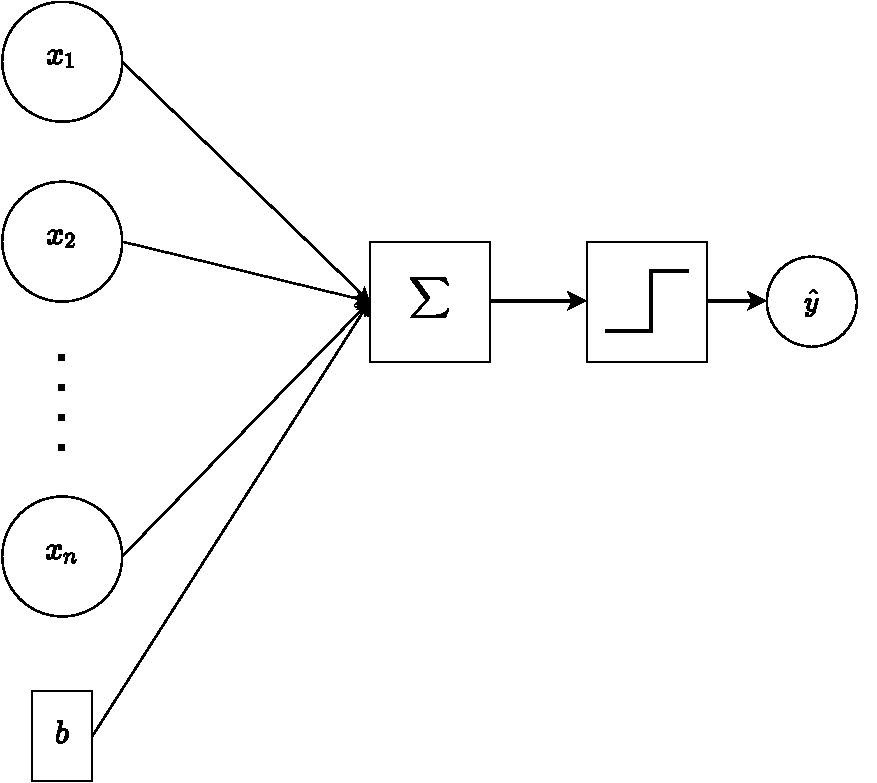
\includegraphics[width=.5\linewidth]{images/perceptron.pdf}
        \caption{Perceptron}
        \label{fig:perceptron}
    \end{figure}
    
    The results then compared with the original output $y_i$ in the
    dataset to learn the correct parameter weight $\mathbf{w}$ and
    bias $b$ by using backpropagation algorithm. The algorithm defines
    a cost function and calculate the gradient of the current cost,
    then the gradient information is processed by another algorithm
    called stochastic gradient descent to try to find the optimal
    parameters that produced the minimum cost. If $\mathbf{\hat{y}} =
    f(\mathbf{x}, \mathbf{W}) = \mathbf{x} \cdot \mathbf{W}$ and the
    cost $z = J(\mathbf{y})$, the simple calculation of the gradient
    can be calculated as follows,
    \begin{align}
        \label{eq:gradient1}
        \frac{\partial z}{\partial x_i} &= \sum_j \frac{\partial z}{\partial y_j} \frac{\partial y_j}{\partial x_i}\\
        \label{eq:gradient2}        
        &= \sum_j \frac{\partial z}{\partial y_j} \sum_k w_k
    \end{align}
    The correction on parameter $\mathbf{W}$ can be calculated by
    following calculation with some learning parameter $\eta$ as shown
    on equation \ref{eq:sgd}.
    \begin{align}
        \label{eq:sgd}
        \hat{w_i} = -\frac{\partial z}{\partial x_i} \times \eta \times w_i
    \end{align}
    Notice that the gradient in equation \ref{eq:sgd} is multiplied by
    $-1$ because the gradient points uphill and to find the minimum
    cost, the parameters needs to traverse downhill on the cost
    function. The learning parameter $\eta$ act as penalization factor
    for the gradient to avoid jumping over the optimal solution.
    Generally, $\eta$ is set to be near zero.
    
    On the development of perceptron, it is clear that model
    consisting of single layer of input and single layer of output
    does not enough to solve XOR problem
    \citep{Goodfellow-et-al-2016}, since what perceptron does is
    separating the space with a hyperplane, or in XOR problem a
    hyperline as shown on figure \ref{fig:xor}. 
    \begin{figure}
        \centering
        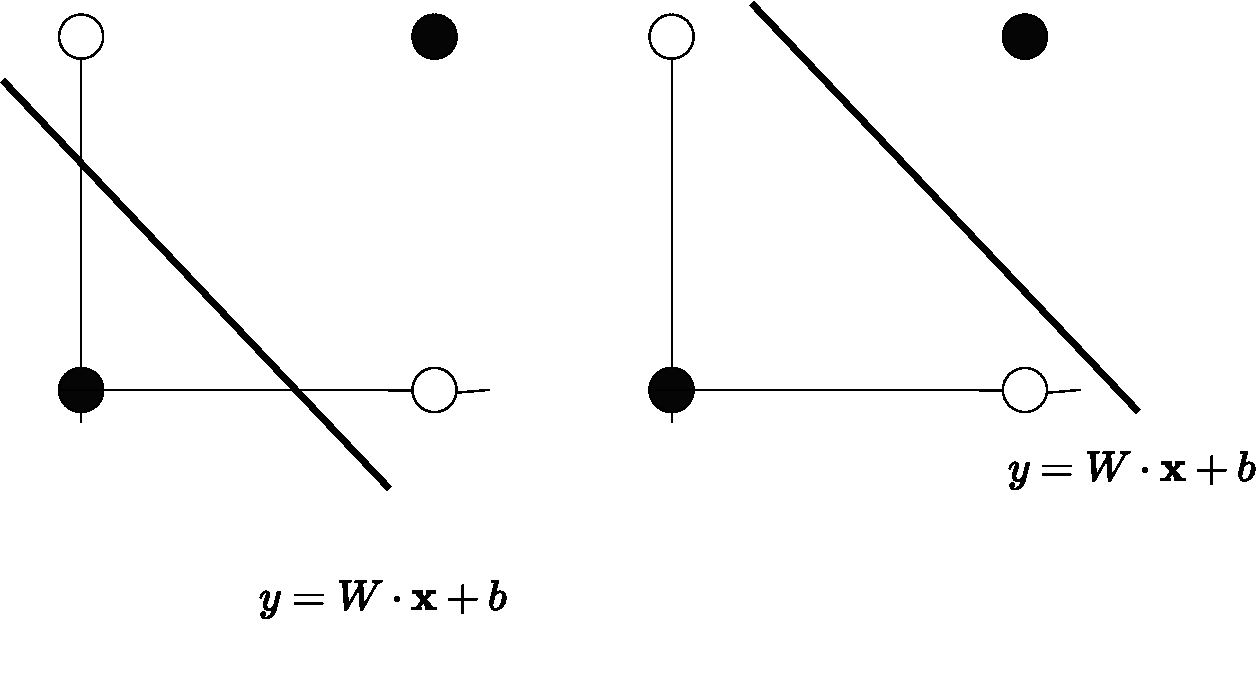
\includegraphics[width=.7\linewidth]{images/xor.pdf}
        \caption{XOR Problem}
        \label{fig:xor}
    \end{figure}
    Thus multilayer perceptron were introduced. This model consist of
    single layer of input, single layer of output, and one or more
    hidden layer. On top of that, more non-linear activation function
    were introduced. Some of those are sigmoid, tanh, rectified linear
    unit (ReLU), and softmax described in equation \ref{eq:sigmoid}
    until \ref{eq:softmax}.

    \begin{align}
        \label{eq:sigmoid}
        \sigma(x) &= \frac{1}{1+e^{-x}} \\
        \label{eq:tanh}
        tanh(x) &= \frac{e^x-e^{-x}}{e^x + e^{-x}}\\
        \label{eq:relu}
        ReLU(x) &= x^+ = max(0, x)\\
        \label{eq:softmax}
        softmax(x) &= \frac{e^{x_i}}{\sum_{j=1}^J e^{x_j}}
    \end{align}

\section{Long-short Term Memory}
    \begin{figure}[H]
        \centering
        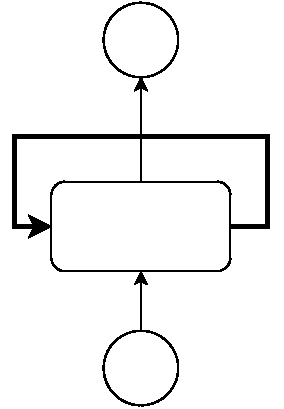
\includegraphics[width=.15\linewidth]{images/rnn.pdf}
        \caption{Recurrent Neural Network}
        \label{fig:rnn}
    \end{figure}
    \begin{figure}[H]
        \centering
        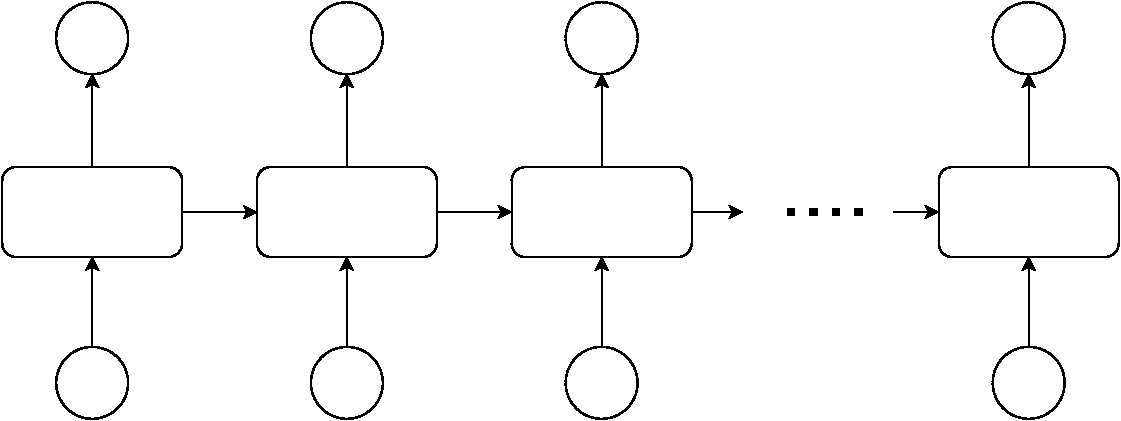
\includegraphics[width=.6\linewidth]{images/unfolded_rnn.pdf}
        \caption{Unfolded Recurrent Neural Network}
        \label{fig:unfolded_rnn}
    \end{figure}
    As aforementioned before, recurrent neural network (RNN) is a
    neural network model that has feedback to its own neuron depicted
    in figure \ref{fig:rnn}. This model used for processing sequential
    data \citep{Goodfellow-et-al-2016}. The idea is given sequence of
    input with length of $t$, $\mathbf{x}_i^{(t)} = x_i^{(1)}, x_i^{(2)},
    \dots, x_i^{(\tau)}$, the input is processed with shared parameter to
    give $t$-lengths output as depicted in figure
    \ref{fig:unfolded_rnn}. Common usage of RNN is for processing
    sentence. For example, given two sentences "I went to Paris in
    2004" and "In 2004 I went to Paris". If we query the model to
    extract information from both sentences and ask when did the
    narrator went to Paris, 2004 would be the relevant information
    regardless when it is appears in a sentence
    \citep{Goodfellow-et-al-2016}. If such task is trained using a
    feedforward neural network that processes fixed size inputs, the
    parameters for each input feature will be separated for each
    sequence. In comparison with feedforward neural network, RNN will
    use the same parameters to process all the input sequence. 

    The problem with RNN is that when given a really long sequence,
    either the gradient calculation will vanish since if weight is
    near zero and is multiplied several times sequentially over time
    and the gradient exploded if the weight is larger than one and it
    will be multiplied several times \citep{Goodfellow-et-al-2016}. Those
    problems making processing long sequence on RNN unfavorable. Hence
    another method called long-short term memory (LSTM) was
    introduced. LSTM was created with idea in mind that some paths
    exist to give gradient ability to flow for long sequence. This was
    achieved by introducing self-loops inside the hidden layer that
    has time-scale mechanism that can change dynamically based on the
    input \citep{Goodfellow-et-al-2016}. New components called cell
    gate $C_t$, forget gate $f_t$, and input gate $i_t$ are introduced
    to let the recurrent network split the graph of the hidden unit
    thus gradient can be flowed longer by depending only from the
    output $o_t$ or from both output and hidden states $o_t$ and $h_t$
    respectively. The cell gate interacts with input $i_t$ and previous
    hidden state $h_{t-1}$ to decide the current hidden state $h_t$.
    The calculation process of LSTM for each time step $t=1$ to
    $t=\tau$ is as follows,
    \begin{align}
        \label{eq:lstm:f_t}
        f_t &= \sigma(W_f \cdot [h_{t-1}, x_t] + b_f) \\
        \label{eq:lstm:i_t}    
        i_t &= \sigma(W_i \cdot [h_{t-1}, x_t] + b_i) \\
        \label{eq:lstm:Cc_t}
        \tilde{C}_t &= tanh(W_C \cdot [h_{t-1}, x_t] + b_C) \\
        \label{eq:lstm:C_t}
        C_t &= f_t \times C_{t-1} + i_t \times \tilde{C}_t \\
        \label{eq:lstm:o_t}
        o_t &= \sigma(W_o \cdot [h_{t-1}, x_t] + b_o) \\
        \label{eq:lstm:h_t}
        h_t &= o_t \times tanh(C_t) \\
        \label{eq:lstm:y_t}
        \hat{y_t} &= softmax(o_t)
    \end{align}
    Cell gate $C_t$ controls the hidden state as described in equation
    \ref{eq:lstm:h_t}. If $C_t = 0$, the hidden state $h_t = 0$,
    meaning the previous information of a certain features is dropped
    for the gated hidden states. The LSTM hidden cell's architecture
    is depicted in figure \ref{fig:lstm}.

    On top of the normal sequence, the reverse sequence can also be
    calculated starting at time step $t=\tau$ to $t = 1$ then the
    output is joined with the forward sequence. This method is called
    bidirectional-LSTM (bi-LSTM) depicted in figure \ref{fig:bilstm}.
    
    \begin{figure}
        \centering
        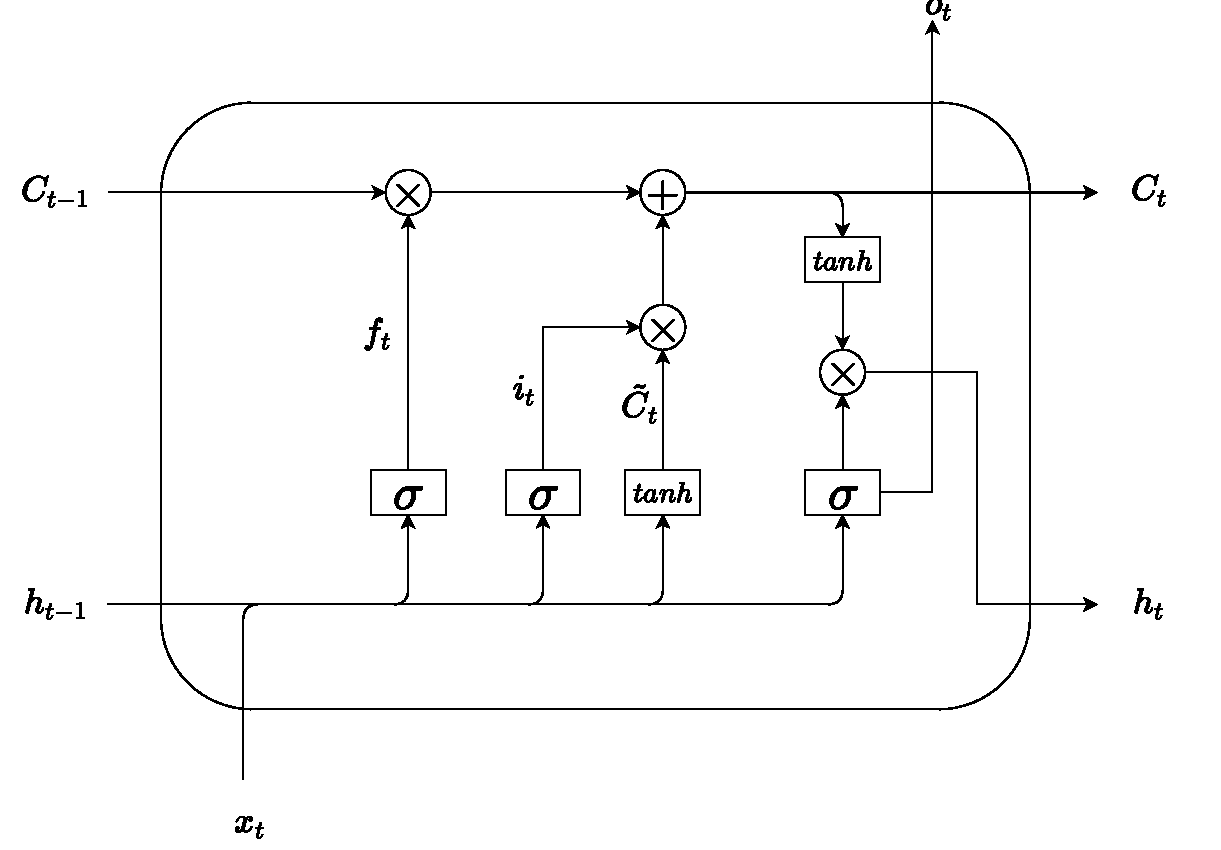
\includegraphics[width=.6\linewidth]{images/lstm.pdf}
        \caption{Gates inside LSTM hidden cell}
        \label{fig:lstm}
    \end{figure}

    \begin{figure}[H]
        \centering
        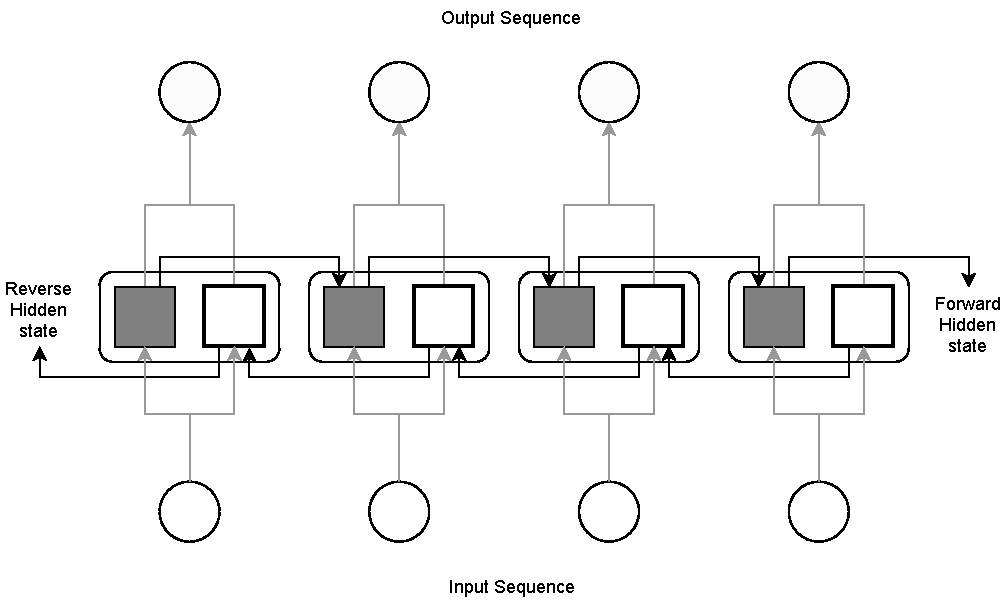
\includegraphics[width=.8\linewidth]{images/bi-lstm.pdf}
        \caption{bi-LSTM with 4 sequence}
        \label{fig:bilstm}
    \end{figure}

\section{Mimick}
    In this research, \textsc{Mimick} is used as baseline model.
    Firstly, pre-trained embedding which contains word $w_i$ and its
    embedding $e_i$ is used as input and target respectively.
    Afterward, the character embedding $g_i \in \mathbf{G}$ for each
    character $c_i \in \mathbf{C}$ was defined. Each word $w_i$ as
    input first broken down into sequence of characters, $w_i = [c_1,
    c_2, \dots, c_n]$, then each character was transformed into its
    embedding, producing sequence of character embeddings $[g_1, g_2,
    \dots, g_n]$. Those character embeddings then fed into bi-LSTM as
    a sequence to extract the features of the word input. The last
    hidden states of both forward $\mathbf{h}_f$ and backward
    $\mathbf{h}_b$ then concatenated and fed into a fully connected
    layer with parameters $\mathbf{T}_h$, $\mathbf{b}_H$,
    $\mathbf{b}_T$ and $\mathbf{O}_T$ and nonlinear function $g$ to
    predict the embedding of the input word as described by equation
    \ref{eq:mimick}.
    \begin{equation}
        \label{eq:mimick}
        f(w) = \mathbf{O}_{T} \cdot g(\mathbf{T}_h \dot [\mathbf{h}_f;
        \mathbf{h}_b] + \mathbf{b}_h) + b_T
    \end{equation}
    The objective of the training is to get the predicted embedding
    $f(w_i)$ as close as the pre-trained word embeddings $e_i$. This
    was done by minimizing the squared Euclidean error,
    \begin{equation}
        \label{eq:mimickloss}
        \mathcal{L} = \Vert f(w_i) - e_i \Vert_2^2
    \end{equation}
    The full process of predicting the embedding $f(w_i)$ is depicted
    in figure \ref{fig:mimick}.
    \begin{figure}
        \centering
        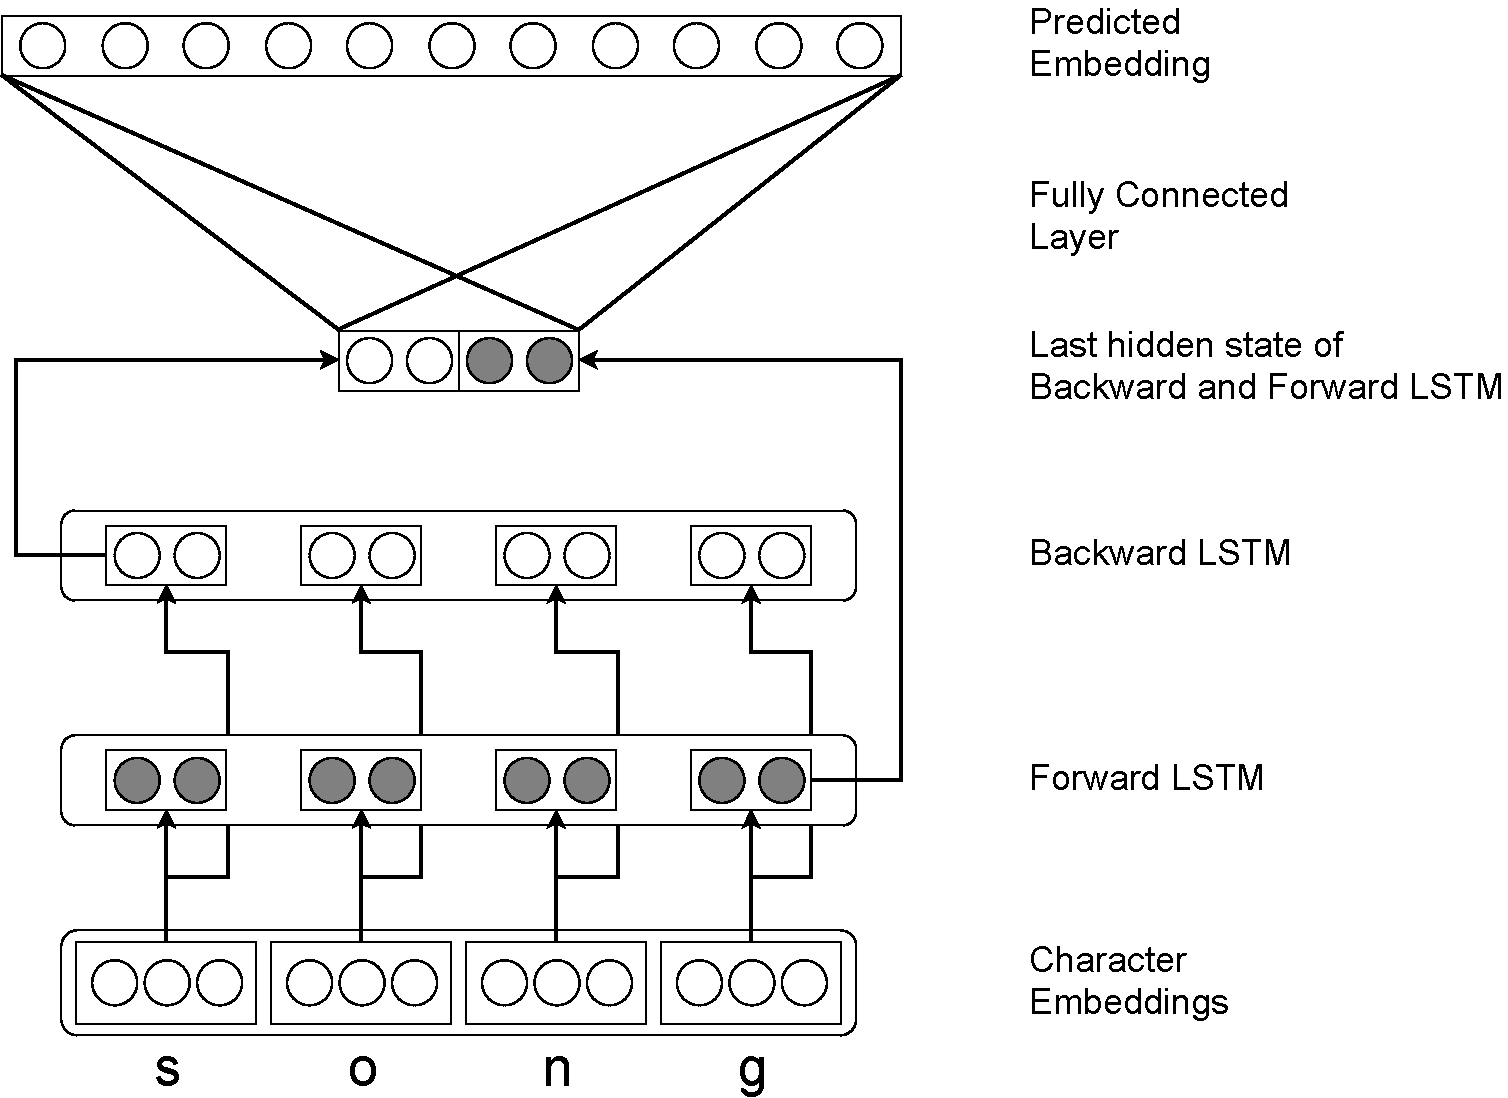
\includegraphics[width=.8\linewidth]{images/mimick.pdf}
        \caption{Mimick architecture}
        \label{fig:mimick}
    \end{figure}

    As aforementioned in the previous section, cell gate $C_t$
    controls which hidden neuron in hidden states at time $t$ will
    pass through to the next sequence. \textsc{Mimick} uses only the
    last hidden state of the bi-LSTM thus increases the chance of the
    early important sequence to be dropped when cell gate $C_t$
    decided to drop the information at certain point when there exist
    some important sequence to trigger the cell gate $C_t$ to drop
    previous information. Although bi-LSTM could serve the purpose to
    include the early sequence, the intermediate important sequence
    that is appears in the middle of two important sequences might
    be dropped because of the cell gate $C_t$ decided to drop previous
    sequence. This problem fueled another approach to be introduced,
    namely using convolutional neural network as the feature extractor
    for the character sequence.

\section{Convolutional Neural Network}
    Convolutional neural network (CNN) is a model that is used to
    process data that has grid topology \citep{Goodfellow-et-al-2016}.
    For a time series data that has a regular time interval, CNN can
    process this as a one-dimensional grid data and for an image data
    CNN can process this as a two-dimensional grid or 3-dimensional
    grid given the number of channel presents on the image data. This
    model concept was first introduced for handwriting recognition
    \citep{generalization1989lecun}.

    In general, convolution is operation of two function, the data and
    the kernel, that is taking values from both function and
    elementwise multiplied was done and then summed to get the total
    overlaps between both function at time $t$. In general, the kernel
    has only limited size that has non zero values while the rest is
    zero. Thus the convolution operation is done locally by processing
    parts of the data several times. To obtain the entirety processed
    data, the kernel needed to be shifted in all direction depending
    on the data dimension. This process is easier to be explained with
    mathematical expression. In equation \ref{eq:conv:2},
    one-dimensional data or function $f(t)$ is being convoluted with a
    kernel $g(t)$.
    \begin{align}
        \label{eq:conv:1}
        h(t) &= (f * g)(t)\\
        \label{eq:conv:2}
        h(t) &= \int_{-\infty}^\infty f(u)g(t-u) du
    \end{align}
    In discrete type signal, the calculation processes becomes as
    shown in equation \ref{eq:conv_d:2}.
    \begin{align}
        \label{eq:conv_d:1}
        h(t) &= (f * g)(t)\\
        \label{eq:conv_d:2}
        h(t) &= \sum_{u = -\infty}^{\infty} f(u)g(t-u)
    \end{align}
    For two-dimensional data, the discrete convolution function
    becomes as shown in equation \ref{eq:conv_d_2d}.
    \begin{align}
        \label{eq:conv_d_2d}
        h[i, j] = \sum_{m = -\infty}^{\infty}\sum_{n = -\infty}^{\infty}f[m, n]\cdot g[i-m, j-n]
    \end{align}

    In CNN, one of the function is the input data and the other is the
    weight. Typically, the weight's, also known as kernel, size is
    smaller than the input data although it is possible to have kernel
    size that is bigger than the input but there is no reason to have
    larger kernel if the objective is to learn local features of the
    data. To process an image data, the image input is convoluted with
    some kernels to produce different spatial features. This features
    then will be processed with a feedforward neural network to
    produce some prediction of classification or regression. The
    convolution process of one patch of an input image is depicted in
    figure \ref{fig:convolution}.
    
    \begin{figure}
        \centering
        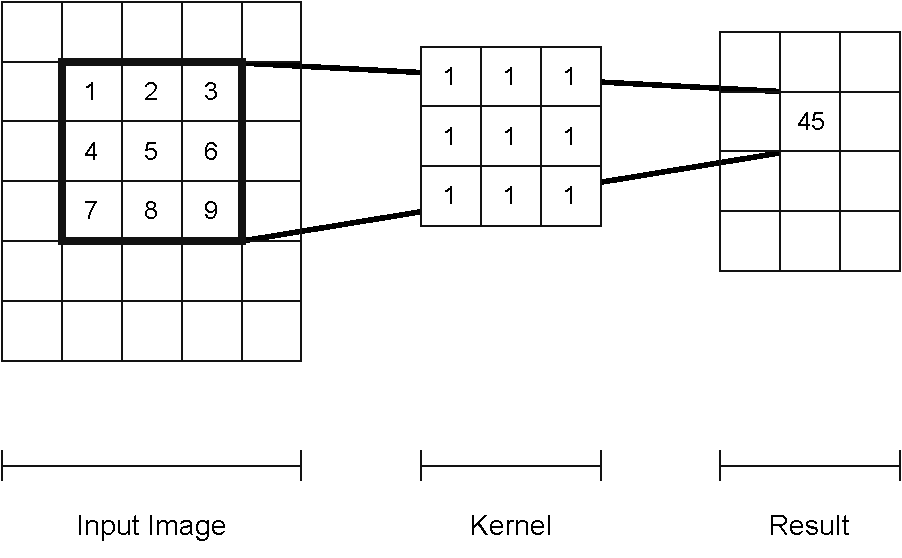
\includegraphics[width=.6\linewidth]{images/convolution.pdf}
        \caption{Convolution process of input image with kernel size $3\times3$}
        \label{fig:convolution}
    \end{figure}
    
    Another intermediate layer that can also be used in CNN called
    maxpooling layer. Maxpooling is a process of finding a maximum
    value inside a given window from a given grid. In CNN, maxpooling
    is used for finding within the input data that gives the highest
    response with a given kernel. Then the process of convolution and
    maxpooling is repeated until desired architecture is produced. The
    process of one patch of an input image is depicted in figure
    \ref{fig:maxpool}. Maxpooling process act as a gate for the
    highest response to receive backward connection for correcting the
    kernel. This is so that only parts of the image that has highest
    response will also corresponds to the correction of the kernel
    while the others treated as less useful. 

    \begin{figure}
        \centering
        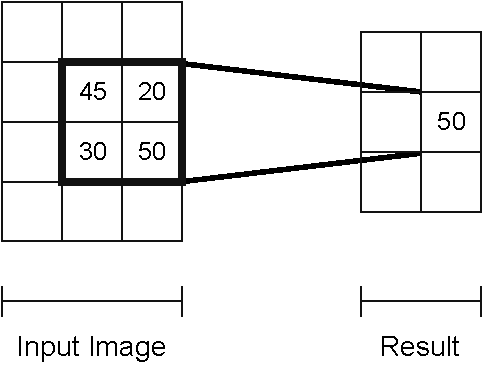
\includegraphics[width=.4\linewidth]{images/maxpool.pdf}
        \caption{Maxpooling process of input image with window size $2\times2$}
        \label{fig:maxpool}
    \end{figure}

    Convolution and maxpool then can be combined together to produce
    features map that act as input to the fully connected network. As
    an example, CNN with two convolution and maxpool architecture is
    depicted in figure \ref{fig:cnn}. In most cases, after doing
    convolution, non-linear activation function are applied.
    
    \begin{figure}
        \centering
        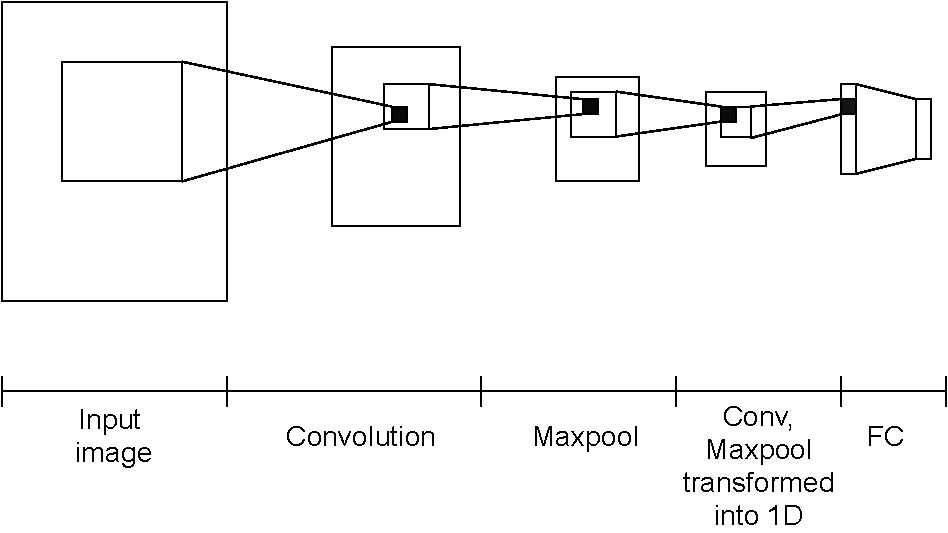
\includegraphics[width=.8\linewidth]{images/cnn.pdf}
        \caption{Example of CNN architecture}
        \label{fig:cnn}
    \end{figure}

\section{N-grams}
    N-grams is a method that is mostly used for word prediction
    \citep{speech2009Jurafsky:2009:SLP:1214993}. Given a sentence,
    \begin{center}
        \texttt{Please do not sit ...}
    \end{center}
    word \textit{on} or \textit{at} is more likely to follow instead
    of \textit{run} or \textit{bacteria}. In short, the previous task
    can be written as $P(w\vert h)$, probability of the next word $w$
    given some history part of sentence $h$. In previous case, the
    history $h$ is "\textit{Please do not sit}" and the probability in
    question is the following word $w$ will be "\textit{on}". To solve
    this task, counting the appearance of history $h$ followed by word
    $w$ can be used to retrieve the probability
    \citep{speech2009Jurafsky:2009:SLP:1214993}. Mathematically it can
    be written as follow,
    \begin{equation*}
        \label{eq:countingprob}
        P(\text{on} \vert \text{Please do not sit}) = 
        \frac{C(\text{Please do not sit on})}{C(\text{Please do not sit})}
    \end{equation*}
    Previous method can give good estimation, but because language is
    creative and new sentences generated every time, everything that
    exist on the internet is not enough to produce good estimate
    \citep{speech2009Jurafsky:2009:SLP:1214993}. On top of that, if
    the joint probability of the sequence would be calculated, there
    will be many estimations where each estimation is not exact
    because there is no way for the probability to be calculated given
    long sequence of preceding words because as stated above,
    language is creative
    \citep{speech2009Jurafsky:2009:SLP:1214993}. Given sequence of
    words $(w_1, w_2, \dots, w_n)$, the joint probability of these
    sequence can be calculated by using chain rule as follows,
    \begin{align}
        \label{eq:jointprob1}
        P(w_1, w_2, \dots, w_n) &= P(w_1)P(w_2 \vert w_1)P(w_3 \vert w_1, w_2) \dots
        P(w_n \vert w_1, w_2, \dots, w_{n-1}) \\
        \label{eq:jointprob2}
        &= \prod_{i=1}^n P(w_i \vert w_1, \dots, w_{i-1})
    \end{align}
    As shown on equation \ref{eq:jointprob1}, each occurrence of
    preceding sequence that followed by the desired word is estimated
    by counting the occurrence as shown in equation
    \ref{eq:countingprob} for the whole history.
    
    Instead of previous calculation, better way to calculate the word
    $W$ given history $h$ is needed because as stated above, language
    is creative making calculating exact probability impossible and
    there will be too many estimation if there is long sequence that
    precedes the target word. Hence n-grams has been introduced to
    approximate the probability of word $w$ from last few sequence of
    the history $h$ instead of a whole
    \citep{speech2009Jurafsky:2009:SLP:1214993}. For instance, only
    two preceding sequences will be taken into calculation.
    In other words, instead of following probability calculation,
    \begin{equation}
        P(\text{on} \vert \text{Please do not sit})
    \end{equation}
    the approximation of the probability will be as follows,
    \begin{equation}
        P(\text{on} \vert \text{not sit})
    \end{equation}
    In other words, the conditional probability then approximated by
    following equation,
    \begin{equation}
        \label{eq:condprobapprox}
        P(w_n \vert w_1, w_2, \dots, w_{n-1}) \approx P(w_n \vert w_{n-2}, w_{n-1})
    \end{equation}
    This approximation method then can be used for joint probability
    approximation as follows,
    \begin{equation}
        P(w_1, w_2, \dots, w_n) = \prod_{i=1}^n P(w_i \vert w_{i-2}, w_{i-1})
    \end{equation}
    for $P(w_j) = 1$ if $j < 1$.

    There are multiple n-grams model that are differentiated by the number
    of sequence used to estimate probability of the next word $w$. For
    example, preceding word in the history $h$ is used for estimating
    the next word $w$ in bigram model and two preceding words in the
    history $h$ is used in trigram model. In general, the window used
    for n-grams are configurable to the needs of the expected results.
    
    Another application of n-grams is that the sequence of character
    is used instead of sequence of words to estimate the probability.
    Differently from word n-grams, character n-grams are able to infer
    the morphological features of a written sentence or words
    \citep{kulmizev-etal-2017-power}. Instead of using history of
    words, character n-grams used history of character to predict the
    next character. All the equation is similar to the word n-gram. On
    top of that, character n-grams are really good for detecting
    patterns in case of typographical error and represented less
    sparsely compared to word n-grams since there are only so much
    character compared to the words made up from existing characters
    \citep{kulmizev-etal-2017-power}.